\documentclass[a4paper,12pt,twoside,openany]{report}
%
% Wzorzec pracy dyplomowej
% J. Starzynski (jstar@iem.pw.edu.pl) na podstawie pracy dyplomowej
% Wersja 0.1 - 8 października 2016
%
\usepackage{polski}
\usepackage{helvet}
\usepackage[T1]{fontenc}
\usepackage{anyfontsize}
\usepackage[utf8]{inputenc}
\usepackage[pdftex]{graphicx}
\usepackage{tabularx}
\usepackage{array}
\usepackage[polish]{babel}
\usepackage{subfigure}
\usepackage{amsfonts}
\usepackage{verbatim}
\usepackage{indentfirst}
\usepackage[pdftex]{hyperref}
\usepackage{amsmath}

% Pakiety oraz kolory pomocnicze do kodu źródłowego.
\usepackage{listings}
\usepackage{color}
\definecolor{dkgreen}{rgb}{0,0.6,0}
\definecolor{gray}{rgb}{0.5,0.5,0.5}
\definecolor{mauve}{rgb}{0.58,0,0.82}
\lstset{frame=tb,
  language=Java,
  aboveskip=3mm,
  belowskip=3mm,
  showstringspaces=false,
  columns=flexible,
  basicstyle={\small\ttfamily},
  numbers=none,
  numberstyle=\tiny\color{gray},
  keywordstyle=\color{blue},
  commentstyle=\color{dkgreen},
  stringstyle=\color{mauve},
  breaklines=true,
  breakatwhitespace=true,
  tabsize=2
}


% rozmaite polecenia pomocnicze
% gdzie rysunki?
\newcommand{\ImgPath}{.}

% oznaczenie rzeczy do zrobienia/poprawienia
\newcommand{\TODO}{\textbf{TODO}}


% wyroznienie slow kluczowych
\newcommand{\tech}{\texttt}

% na oprawe (1.0cm - 0.7cm)*2 = 0.6cm
% na oprawe (1.1cm - 0.7cm)*2 = 0.8cm
%  oddsidemargin lewy margines na nieparzystych stronach
% evensidemargin lewy margines na parzystych stronach
\def\oprawa{1.05cm}
\addtolength{\oddsidemargin}{\oprawa}
\addtolength{\evensidemargin}{-\oprawa}

% table span multirows
\usepackage{multirow}
\usepackage{enumitem}	% enumitem.pdf
\setlist{listparindent=\parindent, parsep=\parskip} % potrzebuje enumitem

%%%%%%%%%%%%%%% Dodatkowe Pakiety %%%%%%%%%%%%%%%%%
\usepackage{prmag2017}   % definiuje komendy opieku,nrindeksu, rodzaj pracy, ...


%%%%%%%%%%%%%%% Strona Tytułowa %%%%%%%%%%%%%%%%%
% To trzeba wypelnic swoimi danymi
\title{Tytuł pracy dyplomowej}

% autor
\author{Jakub Młynarczyk}
\nrindeksu{288226}

\opiekun{dr inż. Łukasz Makowski}
\terminwykonania{1 lutego 2019} % data na oświadczeniu o samodzielności
\rok{2019}


% Podziekowanie - opcjonalne
\podziekowania{
  \noindent
{\Large Podziękowania}
\bigskip

Dziękuję bardzo serdecznie wszystkim pracownikom uczelni, rodzinie oraz pracodawcy za poświęcony czas i energię.

\bigskip

{\raggedleft
Jakub Młynarczyk

}


}

% To sa domyslne wartosci
% - mozna je zmienic, jesli praca jest pisana gdzie indziej niz w ZETiIS
% - mozna je wyrzucic jesli praca jest pisana w ZETiIS
%\miasto{Warszawa}
%\uczelnia{POLITECHNIKA WARSZAWSKA}
%\wydzial{WYDZIAŁ ELEKTRYCZNY}
%\instytut{INSTYTUT ELEKTROTECHNIKI TEORETYCZNEJ\linebreak[1] I~SYSTEMÓW INFORMACYJNO-POMIAROWYCH}
% \zaklad{ZAKŁAD ELEKTROTECHNIKI TEORETYCZNEJ\linebreak[1] I~INFORMATYKI STOSOWANEJ}
%\kierunekstudiow{INFORMATYKA}

% domyslnie praca jest inzynierska, ale po odkomentowaniu ponizszej linii zrobi sie magisterska
\pracamagisterska
%%% koniec od P.W

\opinie{%
  \newpage
\begin{center}
 {\large\bf  Opinia} \\
o pracy dyplomowej magisterskiej wykonanej przez dyplomanta\\
{\bf Zdolnego Studenta i Pracowitego Kolegę} \\
 Wydział Elektryczny, kierunek Informatyka,  Politechnika Warszawska\\
Temat pracy\\
\textit{\bf
TYTUŁ PRACY DYPLOMOWEJ
}\\
\end{center}
\medskip
\noindent
Promotor: {\bf dr inż. Miły Opiekun}\\
Ocena pracy dyplomowej: {\bf bardzo dobry}

\medskip

\centerline{\bf Treść opinii}
   Celem pracy dyplomowej panów dolnego Studenta i Pracowitego Kolegi  było
opracowanie systemu pozwalającego symulować  i opartego o oprogramowanie o
otwartych źródłach (ang. Open Source). Jak piszą Dyplomanci, starali się opracować
system, który łatwo będzie dostosować do zmieniających się dynamicznie wymagań,
będzie miał niewielkie wymagania sprzętowe i umożliwiał dalszą łatwą rozbudowę oraz
dostosowanie go do potrzeb.
Przedstawiona do recenzji praca składa się z krótkiego wstępu jasno i
wyczerpująco opisującego oraz uzasadniającego cel pracy, trzech rozdziałów (2-4)
zawierających opis istniejących podobnych
rozwiązań, komponentów rozpatrywanychjako kandydaci do
tworzonego systemu i wreszcie zagadnień wydajności wirtualnych
rozwiązań. Piąty rozdział to opis przygotowanego przez
Dyplomantów środowiska obejmujący opis konfiguracji
środowiska oraz przykładowe ćwiczenia laboratoryjne. Ostatni
rozdział pracy to opis możliwości dalszego
rozwoju projektu. W ramach przygotowania pracy Dyplomanci zebrali i przedstawili w
bardzo przejrzysty sposób duży zasób informacji, co świadczy o dobrej orientacji
w nowoczesnej i ciągle intensywnie rozwijanej tematyce stanowiącej
zakres pracy i o umiejętności przejrzystego przedstawienia tych
wyników. Praca zawiera dwa dodatki, z których pierwszy obejmuje wyniki
eksperymentów i badań nad wydajnością, a drugi to źródła
skryptów budujących środowisko.

 Dyplomanci dość
dobrze zrealizowali postawione przed nimi zadanie,
wykazali się więc umiejętnością zastosowania w praktyce wiedzy
przedstawionej w rozdziałach 2-4.  Uważam, że cele postawione w założeniach pracy zostały pomyślnie
zrealizowane. Proponuję ocenę bardzo dobrą (5).

\vskip 1cm
{
\raggedleft
(data, podpis)\kern1cm

}
  \newpage
  \newpage
\begin{center}
 {\large\bf  Recenzja } \\
pracy dyplomowej magisterskiej wykonanej przez dyplomanta\\
{\bf Zdolnego Studenta i Pracowitego Kolegę} \\
 Wydział Elektryczny, kierunek Informatyka,  Politechnika Warszawska\\
Temat pracy\\
\textit{\bf
TYTUŁ PRACY DYPLOMOWEJ
}\\
\end{center}
\medskip
\noindent
Recenzent: {\bf prof. nzw. dr hab. inż. Jan Surowy}\\
Ocena pracy dyplomowej: {\bf bardzo dobry}
\medskip


\centerline{\bf Treść recenzji}
   Celem pracy dyplomowej panów dolnego Studenta i Pracowitego Kolegi  było
opracowanie systemu pozwalającego symulować  i opartego o oprogramowanie o
otwartych źródłach (ang. Open Source). Jak piszą Dyplomanci, starali się opracować
system, który łatwo będzie dostosować do zmieniających się dynamicznie wymagań,
będzie miał niewielkie wymagania sprzętowe i umożliwiał dalszą łatwą rozbudowę oraz
dostosowanie go do potrzeb.
Przedstawiona do recenzji praca składa się z krótkiego wstępu jasno i
wyczerpująco opisującego oraz uzasadniającego cel pracy, trzech rozdziałów (2-4)
zawierających bardzo solidny i przejrzysty opis: istniejących podobnych
rozwiązań (rozdz. 2), komponentów rozpatrywanychjako kandydaci do
tworzonego systemu (rozdz. 3) i wreszcie zagadnień wydajności wirtualnych
rozwiązań, zwłaszcza w kontekście współpracy  kilku elementów
 sieci (rozdział 4). Piąty rozdział to opis przygotowanego przez
Dyplomantów środowiska obejmujący opis konfiguracji
środowiska oraz przykładowe ćwiczenia laboratoryjne (5 ćwiczeń). Ostatni, szósty
rozdział pracy to krótkie zakończenie, które wylicza także możliwości dalszego
rozwoju projektu. W ramach przygotowania pracy Dyplomanci zebrali i przedstawili w
bardzo przejrzysty sposób duży zasób informacji o narzędziach, Rozdziały 2, 3 i 4 świadczą o dobrej orientacji
w nowoczesnej i ciągle intensywnie rozwijanej tematyce stanowiącej
zakres pracy i o umiejętności syntetycznego, przejrzystego przedstawienia tych
wyników. Drobne  mankamenty tej części pracy to zbyt skrótowe omawianie
niektórych zagadnień technicznych, zakładające dużą początkową wiedzę czytelnika
i dość niestaranne podejście do powołań na źródła.
Utrudnia to w pewnym stopniu czytanie pracy i zmniejsza jej wartość dydaktyczną
(a ta zdaje się być jednym z celów Autorów), ale jest zrekompensowane zawartością
merytoryczną. Praca zawiera dwa dodatki, z których pierwszy obejmuje wyniki
eksperymentów i badań nad wydajnością, a drugi to źródła
skryptów budujących środowisko. Praca
zawiera niestety dość dużą liczbę drobnych błędów redakcyjnych, ale nie wpływają
one w sposób istotny na na jej czytelność i wartość. W całej pracy przewijają
się samodzielne, zdecydowane wnioski Autorów, które są wynikiem własnych i
oryginalnych badań.  Rozdział 5 i dodatki pracy przekonują mnie, że Dyplomanci dość
dobrze zrealizowali postawione przed nimi zadanie. Pozwala to stwierdzić, że
wykazali się więc także umiejętnością zastosowania w praktyce wiedzy
przedstawionej w rozdziałach 2-4. Kończący pracę rozdział szósty świadczy o
dużym (ale moim zdaniem uzasadnionym) poczuciu własnej wartości i jest
świadectwem własnego, oryginalnego spojrzenia na tematykę przedstawioną w pracy
dyplomowej. Uważam, że cele postawione w założeniach pracy zostały pomyślnie
zrealizowane. Proponuję ocenę bardzo dobrą (5).

\vskip 1cm
{
\raggedleft
(data, podpis)\kern1cm

}
}

\streszczenia{
  \newpage
\begin{center}
\large \bf
Problemy współbieżności w algorytmach węzła sieci czujnikowej na przykładzie modelu w języku Go.
\end{center}

\section*{Streszczenie}
Praca składa się z krótkiego wstępu jasno i wyczerpująco opisującego oraz uzasadniającego cel pracy.
Rozdział drugi `Wykorzystane technologie` opisuje technologie, narzędzia oraz systemu wykorzystane w celu wykonania pracy.
Rozdział trzeci `Bezprzewodowe sieci czujnikowe` przedstawia podstawowe zagadnienia związane z bezprzewodowymi sieci czujników, algorytmami i protokołami
stosowanymi w celach uzyskania lepszej efektywności procesu wymiany informacji.
Rozdział czwarty `Architektura systemu` opisuje wymagania oraz implementację autorskiego systemu środowiska symulacyjnego.
Rozdział piąty `Opracowanie wyników eksperymentów` definiuje zakres testów, prezentuje uzyskane wyniki oraz krótko opisuje uzyskane wartości.
Ostatni rozdział pracy `Podsumowanie` to holistyczny opis uzyskanych wyników, zaobserwowanych zależności w bezprzewodowych sieciach czujnikowych oraz możliwościach dalszego rozwoju projektu. 

\bigskip
{\noindent\bf Słowa kluczowe:} wsn, sieci czujnikowe, golang, LEACH, PEGASIS

\vskip 2cm

\newpage
\begin{center}
\large \bf
Challenges of concurrency in wireless sensor network, based on a model developed in Go.
\end{center}

\section*{Abstract}
This thesis presents a novel way of using a novel algorithm to present complex problems of concurrency in wireless sensor networks. 
In the first chapter briefly presents presents the objectives and goals of the document.
The second chapter describes all available tools, technologies and utilities used in the process of writing.
The third chapter presents the fundamentals of wireless sensor networks and technologies.
The fourth chapter presents requirements and implementation details of custom-made simulation environment written in Go programming language.
The fifth chapter defines a set of tests and sub-tests, as well as presents results of those tests, which enable to compare existing wireless sensor network protocols
and proves the correctness of end-to-end simulator.
Final chapter summarizes all the tests results, discovered dependencies and points some new possibilities of further development of the simulator.

\bigskip
{\noindent\bf Keywords:} wsn, wireless sensor networks, golang, LEACH, PEGASIS

\vfill
}

\begin{document}
\maketitle

%-----------------
% Wstęp
%-----------------
\chapter{Wstęp}

W ciąg ostatnich lat obserwujemy szybki rozwój technologii informatycznych i teleinfromatycznych w zakresie bezprzewodowych sieci czujnikowych.
Pierwsze implementacje bezprzewodowych czujników wykorzystano w celach zbrojeniowych. Aktualnie, możliwości oferowane przez bezprzewodowe 
czujniki znajdują zastosowanie w nieskończonej liczbie aplikacji, zarówno w przemyśle (np. medycynie), jak również w sektorze prywatnym (np. inteligentny dom).

% TODO: spellchecker

\section{Cel pracy}
Celem pracy są badania problemów współbieżności w algorymatch sieci czujnikowej. Praca wykorzystuje 
ogólnie znane i udokumentowane algorytmy umożliwiające
transmitowanie danych w sieci, w których najważniejszym ograniczeniem jest skończona ilość energii czujnika.

Istotnym elementem pracy jest autorski symulator sieci sensorowej, która stanowi podstawowe narzędzie umożliwiąjące implementację oraz testowanie nowych algorytmów.
Aplikacja umożliwia tworzenie symulacji porównujących efekty zastosowania różnych algorytmów transmisji danych, bez potrzeby wykorzystania fizycznych urządzeń.

% \section{Tworzenie projektu}
% TODO: Przenieść na koniec bo to jest podsumowanie - czas przeszły
% Koncepcja i projekt systemu symulującego model bezprzedowowej sieci czujnikowej został opracy przez autora pracy.
% Pierwszym etapem pracy było określenie wymagań oraz funkcjonalności systemu końcowego. Pierwsze szkice dokumentacji były regularnie konsultowane z promotorem pracy.
% Proces ten pozwolił na zebranie szczegółowych wymagań projektowych. W końcowym etapie zbierania wymagań, autor zdecydował się zajął się tworzeniem prototypu systemu symulującego. 
% Prace te pozwoliły na wczesne przetestowanie założeń i pomysłów dotyczących dekompozycji problemu, których efekt zaowocował uproszczeniem całkowitej architektury systemu.
% Projekt zrealizowano w języku Go, przy wykrzystaniu rozszerzonego systmeu kontroli wersji git.

%-----------------
% Wykorzystane technologie
%-----------------
\chapter{Wykorzystane technologie}

Rozdział ten zawiera opis technologii oraz narzędzi wykorzystanych w pracy dyplomowej. 
Przedstawiony zostanie język oprogramowania Go, w którym napisanym zostały najważniejsze komponenty pracy dyplomowej. Rozdział zawiera również
metody i technologie niezbędne do wygenerowania danych wejściowych, technik serializacji danych oraz ich reprezentacji przy wykorzystaniu
Protocol Buffers, GNUPlot, itd.

\section{Język programowania Go}
Go (Golang) to język programistyczny stworzony jako wolne oprogramowanie (open source) na potrzeby firmy Google, Inc. 
Głównymi architektami języka są Robert Griesemer, Rob Pike i Ken Thompson.
Golang umożliwia tworzenie komercyjnego oprogramowania i jest wspierany na wielu sytemach opearcyjnych (Linux, Windows, Mac OS X).

Język Go należy do kategorii języków kompilowanych, z statycznym definiowaniem typu zmiennych. 
Poniżej przedstawiony został fragment kodu źródłowego napisane w języku Go.

\begin{lstlisting}
package main

import (
  "fmt"

  "github.com/golang/example/stringutil"
)

type Label struct {
  Text string
  X, Y int
}

func (l *Label) ReverseText() {
  l.Text = stringutil.Reverse(l.Text)
}

func main() {
  var x = 100
  fmt.Printf("<%T>: %v", x, x)
  // Expected output: <int>: 100
  hello := Label{
    Text: "Hello",
    X:    100,
    Y:    200,
  }
  
  fmt.Println(hello.Text)
  // Expected output: hello
  hello.ReverseText()
  fmt.Println(hello.Text)
  // Expected output: olleh
}

\end{lstlisting}

W powyższym przykładzie przedstawione zostało kilka innowacyjnych funkcjonalności języka Go.
Składnia języka oraz funkcjonalności zbliżone są do C/C++ czy Python, jednakże występuje kilka cech unikatowych dla Go.

\paragraph{Porównanie Go z Python}
\begin{itemize}
 \item Go jest językiem wspomagającym tworzenie aplikacji wielowątkowych.
 \item Go jest językiem statycznym, co pozwala wyeliminować błedy typu runtime wynikające z typu zmiennej.
 \item Go jest językiem samodokumentującym. Określony odgórnie format komentarzy umożliwia automatyczne tworzenie przejrzystej dokumentacji.
 \item Go jest językiem kompilowalnym, co pozwala na szybsze uruchamianie i egzekucję oprogramowania.
 \item Go wykorzystuje mniej pamięci. Przykład: W Go zmienna typu int32 wymaga 4 bajty pamięci, w Python 24 bajty.
 \item Python umożliwia runtime reflection.
 \item Python posiada większy bazę publiczych bibliotek.
\end{itemize}

\paragraph{Porównanie Go z C++}
\begin{itemize}
 \item Go posiada system zarządzania pamięcią (garbage collector).
 \item Go jest językiem wspomagającym tworzenie aplikacji wielowątkowych.
 \item Go jest językiem samodokumentującym. Nie wymaga tworzenia plików typu header.
 \item Go nie jest językiem obiektowym. Zdolność dziedziczenia (inheretance) została zastąpiona osadzaniem (embedding).
 \item Go posiada możliwość użycia (zaimportowania) dowolnej bilbioteki C, C++.
 \item C++ posiada osiągnać szybszą egzekujcę oprogramowania.
 \item C++ posiada tworzenie kodu niezależnie od typu zmiennej (generics).
 \item C++ nie posiada systemu zarządzania pamięcia (garbage collector), co umożliwia większą kontrolę nad zasobami pamięci (np. w mikrokontrolerach).
\end{itemize}

\paragraph{Unikatowe cechy Go}
\begin{itemize}
 \item Produktem kompilacji jest plik egzekucyjny posiadający wszystkie niezbędne zależności.
 \item Zarządzanie pakietami pozwala na importowanie rozwiązań bezpośrednio z GitHub (lub innych serwisów zewnętrznych).
 \item Dynamiczna alokacja typu zmiennej statycznej.
 \item Natywnie wspierane tworzenie oprogramowania wykorzystującego wielowątkowośc i współbieżność procesów.
 \item Natywna metoda testowania funkcjonalności i bibliotek.
 \item Pełny zestaw wbudowanych narzędzi pozwalających na testowanie wydajności kodu (benchmarking), formatowania składni kodu zgodnie ze standardem (gofmt),
       oraz wiele innych funkcjonalności.
\end{itemize}

\section{Serializacja danych Protocol Buffers}
% FIXME: ściana tekstu - brak obrazków
Protocol Buffers (proto, protobuf) to mechanizm serializacji danych stworzony na potrzeby firmy Google, Inc.
Protocol Buffers to mechanizm współpracującym niezależnie od języka oprogramowania aplikacji czy platformy na którym uruchamiana jest aplikacja.
Technologia ta definiuje strukturę danych (proto schema) za pomocą dedykowanego języka, składającego się z prostych zmiennych (np.: int64, string) 
oraz złożonych komunikatów (message). Poniżej przedstawiona została przykładowa struktura.

\begin{lstlisting}
// example.proto
syntax = "proto3";

// Citizen represents a single citizen of Poland.
message Citizen {
  // The name of a citizen.
  string name = 1;
  // The surname of a citizen.
  string surname = 2;
  // (required) Unique Polish national identification number.
  PESEL pesel = 3;
}

// PESEL represents Polish Universal Electronic System for
// Registration of the Population.
message PESEL {
  // (required) Unique Polish national identification number.
  uint64 number = 1;
  bool active = 2;
}
\end{lstlisting}

Struktura ta przechowywana jest w plikach o rozszerzeniu `.proto`, które są następnie kompilowane do dowolnego z wspieranych języków oprogramowania 
(w przypadku Protocol Buffers w wersji 3, wspierana jest generacja kodu w Java, C++, Python, Java Lite, Ruby, JavaScript, Objective-C, C\# oraz PHP).
Następnie, zserializowane dane zostają zapisane w formacie binarnym (wire format), który umożliwia na uzyskanie wyższego poziomu kompresji danych oraz transmisję danych 
bez potrzeby wykonania dalszego kodowania. 
Wynikiem kompilacji plików `.proto` jest zestaw bibliotek zawierający wygenerowany kod źródłowy, wraz z gotowymi strukturami, funkcjami i metodami niezbędnymi do 
operowania danymi w sposób natywny dla wybranego języka programowania.

\section{Nardzędzia dodatkowe}

Sekcja ta przedstawia zestaw narzędzi których funkcjonalności umożliwiły stworzenie oraz ułatwiły zarządzanie oprogramowaniem stworzonym w celach
pracy dyplomowej. 

\subsection{System kontroli wersji git}
Git to rozproszony system kontroli wersji stworzony jako wolne oprogramowanie (open source). 
Głównymi architektem narzędzia jest Linus Torvalds. Git to oprogramowanie powszechnie stosowanym w przypadku zarządzania oprogramowaniem.
Narzędzie to umożliwia tworzenie pobocznych gałęzi (branch) niezależych od głównej gałęzi. Funkcjonalność ta pozwala na niezależne wprowadzanie zmian
w kodzie na określonej wersji kontrolej, które mogą następnie zostać wprowadzon ponownie do gałęzi głównej (merge).
Architektura rozproszna git (w przeciwieństwie do zcentralizowanych systemów kontroli wersji) umożliwia programistom na posiadanie lokalnej kopii repozytorium,
której zmiany mogą zostać następnie wprowadzone do gałęźi głównej.

\subsection{GNUPlot}

GNUPlot to narzędzie do generowania wykresów funkcji w oparciu o dane wejściowe. Program dostępny jest niemal na każdym systemie operacyjnym.
Przy pomocy GNUPlot generować można dwu- oraz trzywymiarowe wykresy, które zapisane mogą zostać w różnych formatach t.j. PNG, SVG czy JPEG.

\subsection{Docker}

Docker to narzędzie stworzone jako wolne oprogramowanie (open source) napisane w języku Go przez firmę Docker, Inc.
Narzędzie to pozwala na tworzenie kontenerów, które izolują aplikację na poziomie systmeu operacyjnego. W przeciwieństwie do maszyn wirtualnych, kontener nie wymaga
wirtualizowania systemu operacyjnego dla każdego z kontenerów. Wszystkie równolegle działające kontenery aplikacji działające na pojedynczym urządzeniu współdzielą
parametry fizyczne maszyny oraz jądro systemu operacyjnego (np. Linux). Izolacja kontenerów widoczna jest na poziomie zależności (dependency) do określonych wersji
bibliotek (libraries), narzędzi (binaries), plików konfiguracyjnych czy parametrów.

%-----------------
% Teoria bezprzewodowych sieci sensorowych
%-----------------
\chapter{Bezprzewodowe sieci czujnikowe}

W tym rodziale przedstawiona zostanie najważniejsza część teoretyczna bezprzewodowych sieci sensorych, która jest niezbędna w celu zrozumienia problemu
rozwiązywanego w pracy dyplomowej.

\section{Wstęp do bezprzewodowych sieci sensorowych}
Bezprzewodowe sieci sensorowe (wireless sensor network) nazywa się również bezprzewodowymi sieciami czujników.
Sieć czujnikowa składa się z urzadzeń, których funkcją jest realizowanie określonego zadania.
Pierwsze aplikacje i zastosowania bezprzewodowych sieci czujników zostały wdrożone na potrzeby wojskowe, jednakże przeciągu ostatnich lat, technologie te znalazły
wiele nowych zastosowań w przemyśle (np. pomiary meteorologiczne) i aplikacjach codziennych (np. systemy domów inteligentnych).

Rozwój technologii, malejący koszt elektroniki oraz dostępność produktów bezprzewodowej sieci czujnikowej, umożliwia tworzenie dedykowanych aplikacji.
Na rynku dostępnych jest wiele urządzeń oraz rozwiązań, a proces wyboru uzależniony jest przede wszystkim od wymogów projektu oraz budżetu.
Dla uproszczenia przyjąć można, że pojedynczy czujnik powinien składać się z procesora zdolnego wykonywać określone zadanie, pamięci zdolnej do przechowywania informacji
oraz anteny, która umożliwia nadawanie i odbieranie informacji.

Proces wymiany informacji między urządzeniami zależy od protokołów i implementacji.
Niezaleznie jednak od protokołu i implementacji, cel pozostaje niezmienny. Informacje posiadane przez węzeł w sieci (np. pomiar temperatury otoczenia) musza zostać przekazane z węzła pomiarowego 
do węzła głównego. Węzeł główny, zwany również `sink` jest odpowiedzialnym za agregację wszystkich informacji oraz ich dalsze przetwarzanie.  
W dalszej części pracy, przedstawione zostaną dwa protokoły trasowania (routingu), których zadaniem jest zoptymalizowanie energetyczne procesu komunikacji, podwyższenie niezawodności systemu 
oraz umożliwienie zautomatyzowanej organizacji topologii sieci.
By móc zrozumieć istotę i korzyści wykorzystania protokołów trasowania, niezbędnym jest przedstawienie najprostrzego schematu komunikacji, komunikacji bezpośredniej.

\section{Model transmisji}

% TODO w komentarzu się ładnie koloruje w edytorze Kile (polecam)
 * Koszt transmisji
 * Założenia dotyczące opóźnień i innych parametrów

\section{Protokoły}

\subsection{Komunikacja bezpośrednia}

Komunikacja bezpośrednia jest rozwiązaniem najprostrzym z perspektywy implementacji, jednakże nieefektywnym z poziomu energetycznego. 
Węzły znajdujące się sieci nie są zaangażowane w podejmowanie decyzji dotyczących optymalizacji kosztów transmisji. 
Adres węzła głównego (sink) może być zaprogramowany na poziomie pliku konfiguracyjnego.
Dane wysyłane przez węzeł nadawane są bezpośrednio do węzła głównego.
Model środowiska symulacyjnego definiuje koszt transmisji komunikacji. Wartość ta zależna jest od odległości między dwoma węzłami.
Czas życia węzłów (posiadających identyczną ilość energii początkowej oraz wielkość przesyłanych informacji) wydłuża się, wraz z malejącym dystansem do węzła głównego.

Poniższa ilustracja przedstawia trzy węzły w sieci, które komunikują się bezpośrednio z węzłem głównym:

\begin{figure}
 \centering
 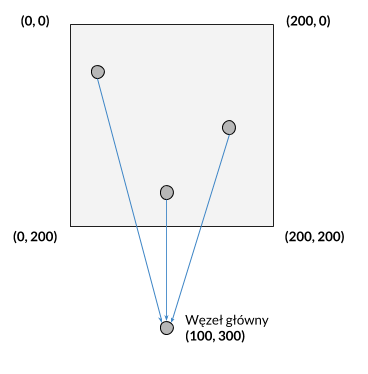
\includegraphics[width=10cm]{images/komunikacja_bezposrednia.png} 
\end{figure}

\subsection{LEACH}

LEACH (Low-Energy Adaptive Clustering Hierarchy) jest algorytmem wykorzystywanych w protokołach routingu bezprzewodowej sieci czujnikowej.
W przeciwieństwie do komunikacji bezpośredniej, LEACH jest protokołem w którym występuje hierarchia. 

Zestaw operacji w protokole LEACH nazywa się rundami (round). Każda z rund podzielona jest na dwie fazy.
W pierwszej fazie, fazie konfiguracyjnej (setup), węzły dokonują podziału sieci na niezależne klastry (cluster).
W drugiej fazie, fazie komunikacyjnej (steady state), węzły uczestniczące w sieci dokonują wymiany informacji za pomoca agregacji danych w klustrze, które następnie
przesłane są do stacji bazowej.

Faza konfiguracji (setup) zbudowana jest z trzech etapów.
W pierwszym etapie węzły dokonują wyboru roli w rundzie. W LEACH występują dwa rodzaje węzłów:

\begin{itemize}
 \item węzły typu cluster head (CH)
 \item węzły standardowe (non-CH)
\end{itemize}

Każdy z węzłów generuje losową wartość `n` z zakresu [0, 1]. Wartość ta podstawiona w poniższe równanie:

\[
T(n) = \begin{cases}
\frac{P}{1 - P[r * mod(1/P)]} & \text{jeżeli } n \in G\\
0 & \text{w innym przypadku}
\end{cases}
\]

gdzie P oznacza wartość z zakresu (0, 1] definiujaca prawdopodobięństwa wyznaczenia węzła typu cluster head.
G jest zbiorem węzłów które nie pełniły roli cluster head w ostatnich 1/P rundach.

W momencie ustalenia roli przez węzły, każdy z węzłów informuje pozostałe węzły uczestniczące w sieci o swojej roli w rundzie.

Kolejnym etapem fazy konfiguracji jest wyznaczenie klustra do którego zostaną przyłączone węzły standardowe.
Każdy z węzłów standardowych wybiera jeden węzeł typu cluster head. W przypadku otrzymania informacji od kilku węzłów typu cluster head,
węzeł standardowy wybiera węzeł CH znajdujący się najbliższej (węzeł którego sygnał jest najmocniejszy).

Ostatnim etapem jest ukończenie formowania klusterów w którym znajduje się dokładnie jeden węzeł typu cluster head.
Wystąpić może sytuacja w której węzeł typu cluster head nie posiada przynależących węzłów standardowych.
Pozytywnie zakończona faza formowania klastrów tworzy stabilną sieci wymiany informacji.

W tym momencie rozpoczyna się faza komunikacji (steady state) w której węzły standardowe dokonują transmisji danych do  węzła typu cluster head.
Węzły CH dokonują agregacji zebranch informacji oraz bezpośrednie przekazanie ich do węzła głównego (sink).
Stworzenie środowiska w którym węzły dokonują pośredniczenia informacji, pozwala na ograniczenie kosztów energetycznych transmisji danych przez
standardowe węzły (dystans do węzła typu cluster head jest mniejszy niż do sink). Należy jednak pamiętać, że koszt energetyczny transmisji węzłów typu cluster head rośnie, gdyż
stają się one odpowiedzialne za odbieranie informacji, przetworzenie ich, a następnie wysłanie do całości do sink. Wielkość informacji (mierzona w bajtach), przetransmitowana 
z węzłów typu cluster head jest zależna od ilości standardowych węzłów przynależących do CH oraz metody agregacji informacji.

Poniższa ilustracja przedstawia zestaw węzłów w sieci, które wykorzystują protokół LEACH:

%FIXME: For some reason this picture is not located in the correct place.
\begin{figure}
 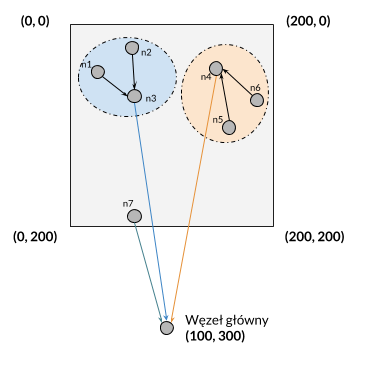
\includegraphics[width=10cm]{images/komunikacja_leach.png} 
\end{figure}

\subsection{PEGASIS}

PEGASIS (Power-Efficient GAathering in Sensor Information Systems) jest algorytmem wykorzystywanym w protokołach routingu bezprzewodowej sieci czujnikowej.
Sieci czujnikowa w której znajdują się węzły o ograniczonej energii (zasilane bateryjnie)

% TODO

%-----------------
% Architektura systemu
%-----------------
\chapter{Architektura systemu}
% TODO: ten rozdział ``robi robotę'' - pozytywnie się wyróżnia ale nadal kilka poniższych subsection
% wymaga poprawy - albo rozbudować albo skonsolidować

System informatyczny stworzony na potrzeby pracy dyplomowej ma za zadanie dostarczenie wyników oraz wykresów niezbędnych do zbadania poniższych zależnożci sprawności energetycznej 
węzłów dla wybranych algorytmów w sieci WSN (komunikacji bezpośredniej, LEACH, PEGASIS).

\section{Komponenty systemu}

Poniższy diagram przedstawia dekompozycję modułów, całkowitą architekturę systemu oraz kierunki interakcji i przepływu informacji.

%TODO Diagram

\subsection{Plik konfiguracyjny}

Plik konfiguracyjny (config file) posiada dane wejściowe pozwalające na zbudowanie środowiska testowego. 
Informacje zawarte w pliku konfiguracyjnym można podzielić na dwie sekcje:

\begin{itemize}
 \item konfiguracja symulatora i sieci
 \item konfiguracja węzła
\end{itemize}

\subsubsection{Konfiguracja symulatora i sieci}

Konfiguracja symulatora i sieci składa się z pięciu zmiennych w komunikacie Config. Każda z tych wartości może być modyfikowana bez potrzeby
ponownej kompilacji oprogramowania symulacyjnego. Poniższa lista przedstawia oraz opisuje znaczenie poszczególnych parametrów konfiguracyjnych:

\begin{itemize}
 \item protokoł (protocol) - zmienna ta zdefiniowana za pomocą komunikatu typu enum E\_Protocol pozwala symulatorowi wybrać odpowiedni 
       protokół sterujący symulacją. Dokładny opis działania protokołów zostanie przedstawiony w dalszej części pracy.
 \item wartości maksymalnej rund pomiarowych (max\_rounds) - zmienna ta pozwala określić wartość rund pomiarowych aktywnych węzłów w pojedynczej symulacji, 
       po której całkowity przebieg symulacji zostanie zatrzymany.
       Wyznaczenie tej wartości umożliwia użytkownikowi określenie dowolnej granicy, bez potrzeby oczekiwania na zakończenie symulacji (wykorzystanie 
       całkowitej energii dostępnej przez węzły pomiarowe).
 \item proporcji węzłów typu kluster do wszystkich węzłów (p\_cluster\_heads) - zmienna ta pozwala określić stosunek ilości węzłów pomiarowych 
       odpowiedzialnych za pośredniczenie w przesyłaniu danych pomiarowych (klastrów) do ilości wszystkich węzłów w sieci. Parametr ten wykorzystywany jest
       zależnie od protokołu.
 \item długość wiadomości (msg\_length) - zmienna ta określa całkowity rozmiar wiadomości generowanych przez pojedynczy węzeł pomiary.
       Długośc wyrażona jest w bajtach i jest sumą dwóch elementów, danych pomiarowych oraz dodatkowych danych generowanych w procesie enkapsulacji
       (np. adresowanie, preambuły, itd.)
 \item konfiguracja węzłów (nodes) - zmienna ta zdefiniowana za pomocą listy komunikatów typu Node. Symulacja musi składać się przynajmniej z dwóch węzłów.
       Kolejność listy ma znaczenie, gdyż pierwszy węzeł pełni rolę głównego odbiornika danych (sink).
       Dokładniejszy opis parametrów poszeczególnych węzłów przedstawiony został w kolejnym porozdziale `Konfiguracja węzła`. 
\end{itemize}

Poniżej przedstawiony został fragment pliku konfiguracyjnego dla konfiguracji symulatora i sieci:

\begin{lstlisting}
enum E_Protocol {
  UNSET = 0;
  DIRECT = 1;
  LEACH = 2;
  APTEEN = 3;
  PEGASIS = 4;
}

message Config {
  // Simulation protocol.
  E_Protocol protocol = 1;
  // Number of maximum rounds in simulation. 
  int64 max_rounds = 2;
  // Percentage of cluster heads among all nodes [0, 1].
  double p_cluster_heads = 3;
  // Size of data sent by individual node (in Bytes).
  int64 msg_length = 4;
  // Nodes points to configuration for each node.
  repeated Node nodes = 5;
}
\end{lstlisting}

\subsubsection{Konfiguracja węzła}

Konfiguracja węzła składa się z pięciu zmiennych w komunikacje Node. Każda z tych wartości może być modyfikowana bez potrzeby
ponownej kompilacji oprogramowania symulacyjnego. Poniższa lista przedstawia oraz opisuje znaczenie poszczególnych parametrów konfiguracyjnych:

\begin{itemize}
 \item indeks (id) - zmienna ta określa unikatowy identyfikator węzła. Parametr ten umożliwia identyfikację węzła podczas symulacji.
 \item energia początkowa (initial\_energy) - zmienna ta określa ilość energii (mierzonej w [J]), którą posiada węzeł w momencie rozpoczęcia symulacji.
       W przypadku zdefiniowania zerowej energii początkowej, węzeł nie będzie brał udziału w komunikacji ze względu na brak zasobów energetycznych na
       przeprowadzenia jakiejkolwiek operacji.
 \item pozycja (location) - zmienna ta zdefiniowana za pomocą komunikatu typu Location pozwala symulatorowi na umieszenie węzła w dwuwymiarowej przestrzenii.
       Pozycja węzła wykorzystywana jest do określania odległości między węzłami i aplikowania kosztów energetycznych operacji (np. transmisji danych).
 \item koszt energetyczny (energy\_cost) - zmienna ta zdefiniowana za pomocą komunikatu typu EnergyCost pozwala na wprowadzenie dodatkowych kosztów energetycznych
       operacji dla poszczególnych węzłów. Podstawowy model posiada ogórnie zdefiniowane koszty energetyczne (model przedstawiony w sekcji TODO).
       W przypadku zdefiniowana zmiennej EnergyCost dla węzła, koszt operacji (np. transmisji, odbioru, pomiaru i przetwarzania danych) ulega zmianie.
 \item opóźnienia czasowe (time\_delay) - zmienna ta zdefiniowana za pomocą komunikatu typu TimeDelay pozwala symulatorowi na wprowadzenie dodatkowych parametrów czasowych
       dla operacji wykonywanych przez węzeł. Iloczyn zmiennej (np. czasu przetwarzania danych węzła [ns]) i kosztu energetycznego działania węzła [J/s] 
       reprezentuje dodatkowe parametry symulacji, które umożliwiają tworzenie zaawansowanych i precyzyjnych scenariuszy.
\end{itemize}

Poniżej przedstawiony został fragment pliku konfiguracyjnego dla konfiguracji węzła:

\begin{lstlisting}
// Node defines a configuration for a single node.
message Node {
  // Unique ID for a node.
  int64 id = 1;
  // Initial value of energy (in Joules). 
  double initial_energy = 2;

  // Location of a node in 2D space.
  Location location = 3;
  // Energy consumption of node operations.
  EnergyCost energy_cost = 4;
  // Time delays introduced by node operations
  TimeDelay time_delay = 5;
}
\end{lstlisting}

Poniżej przedstawiony został fragment pliku konfiguracyjnego dla konfiguracji lokalizacji węzła:

\begin{lstlisting}
// Location defines a X, Y coordinates of a node.
message Location {
  double X = 1;
  double Y = 2;
}
\end{lstlisting}

Poniżej przedstawiony został fragment pliku konfiguracyjnego dla konfiguracji kosztów energetycznych pracy węzła:

\begin{lstlisting}
// EnergyCost defines energy consumption for common node operations.
message EnergyCost {
  // Energy required to transmit one byte (in Joules).
  double transmit = 1;
  // Energy required to receive one byte (in Joules).
  double receive = 2;
  // Energy required to listen the channel for a second (in Joules).
  double listen = 3;
  // Energy required to process sensor data (in Joules).
  double sensor_data_process = 4;
  // Energy required to wake up MCU (in Joules).
  double wake_up_mcu = 5;
}
\end{lstlisting}

Poniżej przedstawiony został fragment pliku konfiguracyjnego dla konfiguracji opóźnień czasowych pracy węzła:

\begin{lstlisting}
// TimeDelay defines time delays for common node operations.
message TimeDelay {
  // Time required to process sensor data (in nanoseconds).
  int64 sensor_data_process = 1;
  // Time required to wake up MCU (in nanoseconds).
  int64 wake_up_mcu = 2;
}
\end{lstlisting}

\subsection{Moduł główny (Core)}

Moduł główny posiada najważniejsze cechy i funkcjonalności umożliwiające modelowanie systemu symulatora WSN.
Wszystkie zaimplementowane struktury (structs) znajdują się w jednej bibliotece (package) o nazwie `core`.

\subsubsection{Węzeł (Node)}

Węzeł (Node) reprezentuje model węzła, będącego elementem podstawowym w sieci. Struktura ta przechowuje dane konfiguracyjne węzła,
poziom energii czy dane historyczne, pozwalające na monitorowanie pracy oraz tworzenie grafów.

Poniżej przedstawiona została struktura węzła oraz definicje funkcji przynależące do struktury.

\begin{lstlisting}
type Node struct {
  Conf    config.Node
  Ready   bool
  nextHop *Node   // As a default set to Base Station.
  Energy  float64 // Energy level of a node.

  transmitQueue int64
  receiveQueue  int64
  // Statistics and aggregation variables.
  dataSent     int64
  dataReceived int64
}

func (n *Node) Transmit(msg int64, dst *Node) error
func (n *Node) Receive(msg int64, src *Node) error
func (n *Node) Info() string

func (n *Node) distance(dst *Node) float64
func (n *Node) consume(e float64) error
\end{lstlisting}

Poniższa lista przedstawia oraz opisuje znaczenie poszczególnych zmiennych struktury węzła (Node):

\begin{itemize}
 \item konfiguracja (Conf) - zmienna publiczna przechowuje konfigurację węzła w formacie protocol buffer (szczegółowe informacje dostępne w `Konfiguracja węzła`).
 \item gotowość (Ready) - zmienna publiczna przechowuje stan gotowości węzła. Wartość `true` oznacza, że węzeł jest gotowy do nadawania i odbierania informacji.
 \item następny skok (nextHop) - zmienna prywatna przechowuje adres do zmiennej węzła, będącego odbiorcą informacji nadawanych przez węzeł. Wartością domyślna w momencie
       rozpoczęcia symulacji jest adres głównego odbiornika danych (sink).
 \item energia (Energy) - zmienna publiczna przechowuje aktualny stan energetyczny węzła. W przypadku wyczerpania energii, zmienna Ready zostaje ustawiona na `false`.
 \item kolejka nadawania (transmitQueue) - zmienna prywatna przechowuje informację o ilości bajtów gotowych do przekazania do następnego węzła na końcu rundy.
 \item kolejka odbioru (receiveQueue) - zmienna prywatna przechowuje informację o ilości bajtów odebranych przez węzeł na początku rundy.
 \item dane nadane (dataSent) - zmienna prywatna przechowuje sumę bajtów nadanych przez węzeł.
 \item dane odebrane (dataReceived) - zmienna prywatna przechowuje sumę bajtów odebranych przez węzeł.
\end{itemize}

Poniższa lista przedstawia oraz opisuje znaczenie poszczególnych funkcji węzła (Node):

\begin{itemize}
 \item Transmit - funkcja pozwala na transmisję danych do węzła.
 \item Receive - funkcja pozwala na odbieranie danych przez węzeł.
 \item Info - funkcja generuje ciąg znaków w podstawowymi informacjami na temat węzła.
 \item distance - funkcja wyznacza wartość odległości pomiędzy dwoma węzłami.
 \item consume - funkcja obciąża energetycznie węzeł.
\end{itemize}

\subsubsection{Sieć (Network)}

Sieć (Network) reprezentuje model środowiska w którym odbywa się symulacja. Struktura ta przechowuje kontroluje przepływ informacji pomiędzy węzłami,
zbiera i eksportuje informacje z poszczególnych rund.

Poniżej przedstawiona została struktura sieci oraz definicje funkcji przynależące do struktury.

\begin{lstlisting}
type Network struct {
  Protocol    Protocol
  BaseStation *Node
  Nodes       sync.Map

  Round     int64
  MaxRounds int64
  MsgLength int64

  GNUPlotNodes       []string
  GNUPlotTotalEnergy []string

  PlotTotalEnergy   *plot.Plot // An amount of total energy in the network per Round.
  PlotNodes         *plot.Plot // A number of alive nodes in the network per Round.
  NodesAlivePoints  plotter.XYs
  NodesEnergyPoints map[int64]plotter.XYs
}

func (net *Network) AddNode(n *Node) error
func (net *Network) Simulate() error
func (net *Network) CheckNodes() int
func (net *Network) PopulateEnergyPoints()
func (net *Network) PopulateNodesAlivePoints()
\end{lstlisting}

Poniższa lista pzedstawia oraz opisuje znaczenie poszeczególnych zmiennych struktury sieci (Network):

\begin{itemize}
 \item protokół (Protocol) - zmienna publiczna przechowuje obiekt definiujący protokół komunikacji pomiędzy węzłami.
 \item stacja bazowa (BaseStation) - zmienna publiczna przechowuje obiekt węzła głównego (sink).
 \item węzły (Nodes) - zmienna publiczna przechowuje obiekty węzłów w sieci. Implementacja przy wykorzystaniu dziennika (hashmap), 
       który umożliwia operacje zapisu i odczytu w procesach równoległych. Kluczem dziennika jest unikatowy identyfikator węzła.
 \item runda (Round) - zmienna publiczna przechowuje numer aktualnej rundy symulacji.
 \item maksymalna ilość rund (MaxRounds) - zmienna publiczna przechowuje maksymalną ilość rund symulacji. 
       W przypadku osiągnęcia wartości Round równej MaxRounds, symulacja zostanie przerwana.
 \item długość wiadomości (MsgLength) - zmienna publiczna przechowuje informację o całkowitej wielkości wiadomości (mierzonej w bajtach) jaka generowana
       jest podczas rundy przez każdy z węzłów. W skład tej wartości wchodzią dane pomiarowe i dodatkowy nakład informacji powstały w wyniku enkapsulacji.
 \item GNUPlotNodes, GNUPlotTotalEnergy - zmienne publiczne przechowujące parametry rund wykorzystywane do generowania grafów przy użyciu narzędzia GNUPlot.
 \item PlotTotalEnergy, PlotNodes, NodesAlivePoints, NodesEnergyPoints - zmienne publiczne przechowujące parametry rund wykorzystywane do generowania grafiów
       przy użyciu biblioteki plotter.
\end{itemize}

Poniższa lista przedstawia oraz opisuje znaczenie poszczególnych funkcji węzła (Node):

\begin{itemize}
 \item AddNode - funkcja pozwala na dodanie węzła do sieci.
 \item Simulate - funkcja umożliwia rozpoczęcie symulacji.
 \item CheckNodes - funkcja sprawdza ilość sprawnych węzłów w sieci.
 \item PopulateEnergyPoints - funkcja sprawdza oraz przechowuje stany energetyczne węzłów.
 \item PopulateNodesAlivePoints - funkcja sprawdza oraz przechowuje ilość sprawnych węzłów w sieci.
\end{itemize}

\subsubsection{Protokół (Protocol)}

Protokół (Protocol) reprezentuje model protokołu komunikacji między wezłami.

Poniżej przedstawiona został interfejs protokołu oraz definicje funkcji przynależące do interfejsu.

\begin{lstlisting}
type Protocol interface {
  Setup(net *Network) ([]int64, error)
  SetNodes(int)
  SetClusters(int)
}
\end{lstlisting}

Poniższa lista przedstawia oraz opisuje znaczenie poszczególnych funkcji węzła (Node):

\begin{itemize}
 \item Setup - funkcja konfiguruje węzły w sieci zgodnie z zaimplementowanym protokołem.
 \item SetNodes - funkcja definiuje ilość węzłów w sieci. Wartość ta jest niezbędna do wyznaczania parametrów w protokołach (np. LEACH, PEGASIS).
 \item SetClusters - funkcja definiuje ilość klastrów w sieci. Wartość ta jest niezbędna do wyznaczania parametrów w protokołach (np. LEACH, PEGASIS).
\end{itemize}

Poniższa lista przedstawia zaimplementowane protokoły:

\begin{itemize}
 \item Komunikacja bezpośrednia	(Direct Communication) - wszystkie węzły w sieci komunikują się bezpośrednio z węzłem głównym (sink).
 \item LEACH (LEACH) - wszystkie węzły w sieci komunikują się zgodnie z topologią ustaloną w procesie konfiguracji LEACH.
 \item PEGASIS (PEGASIS) - wszystkie węzły w sieci komunikują się zgodnie z topologią ustaloną w procesie konfiguracji PEGASIS.
\end{itemize}

\subsection{Moduł symulatora (Simulator)}

Symulator (Simulator) odpowiada za tworzenie środowisk symulacyjnych.
Pojedynczy obiekt symulatora pozwala na zbudowanie wielu scenariuszy symulacji, a następnie ich uruchomienie oraz
wygenerowanie metryk. Dane wyjściowe mogą zostać podanne dalszej analizie przy wykorzystaniu zewnętrznych narzędzi (np. GNUPlot).

\begin{lstlisting}
type Simulator struct {
  namespace map[string]bool
  config    map[string]*config.Config
  network   map[string]*core.Network

  plotTotalEnergy *plot.Plot // An amount of total energy in the network per round.
  plotNodes       *plot.Plot // A number of alive nodes in the network per round.
}

func Create() (*Simulator, error)

func (s *Simulator) AddScenario(name string, conf *config.Config) error
func (s *Simulator) Run() error
func (s *Simulator) ExportPlots(filepath string) error
func (s *Simulator) ExportGNUPlots(filepath string) error

func createAndPopulateFile(filepath string, data []string) error
func (s *Simulator) create(name string, conf *config.Config) error
func createPlot(title, x, y string) (*plot.Plot, error)
func (s *Simulator) plotter() error
\end{lstlisting}

Poniższa lista pzedstawia oraz opisuje znaczenie poszeczególnych zmiennych struktury symulatora (Simulator):

\begin{itemize}
 \item przestrzeń nazw (namespace) - zmienna prywatna przechowuje nazwy symulacji, które w jednoznaczy sposób identyfikują sięć i konfigurację.
 \item przestrzeń konfiguracji (config) - zmienna prywatna przechowuje obiekt konfiguracji (Config) dla każdej symulacji. Kluczem dziennika jest nazwa symulacji.
 \item przestrzeń sieci (network) - zmienna prywatna przechowuje obiekt sieci (Network) dla każdej symulacji. Kluczem dziennika jest nazwa symulacji.
\end{itemize}

Poniższa lista przedstawia oraz opisuje znaczenie poszczególnych funkcji symulatora (Simulator):

\begin{itemize}
 \item Setup - funkcja konfiguruje węzły w sieci zgodnie z zaimplementowanym protokołem.
 \item SetNodes - funkcja definiuje ilość węzłów w sieci. Wartość ta jest niezbędna do wyznaczania parametrów w protokołach (np. LEACH, PEGASIS).
 \item SetClusters - funkcja definiuje ilość klastrów w sieci. Wartość ta jest niezbędna do wyznaczania parametrów w protokołach (np. LEACH, PEGASIS).
\end{itemize}

\section{Obsługa systemu}
 
\subsection{Konfiguracja środowiska i kompilacja}

Poprawna konfiguracja środowiska wymaga instalacji niezbędnych bibliotek i pakietów.

\begin{enumerate}
 \item Instalacja kompilatora i bilbiotek Golang w wersji 1.10.1, lub wyższej.
 \item Instalacja kompilatora Protocol Buffer w wersji 3.6, lub wyżej.
\end{enumerate}

Weryfikacja konfiguracji Golang:

\begin{lstlisting}
 ! Poprawna konfiguracja Golang.
 $ which go
 /usr/local/go/bin/go
 $ go version
 go version go1.10.1 linux/amd64
\end{lstlisting}

Weryfikacja konfiguracji protoc:

\begin{lstlisting}
 ! Poprawna konfiguracja protoc.
 $ which protoc
 /usr/local/bin/protoc
 $ protoc -version
 libprotoc 3.6.0
\end{lstlisting}

Proces kompilacji (z poziomu folderu z kodem projektu):

\begin{lstlisting}
 $ pwd
 /home/<username>/go/src/github.com/keadwen/msc_project
 $ go build
 ! Brak błędów powinien utworzyć plik o nazwie msc_project.
\end{lstlisting}

\subsection{Generowanie konfiguracji}

Wcześniej opisany plik konfiguracyjny jest elementem niezbędnym do uruchomienia symulacji.

Przykładowy plik konfiguracjy (example.pbtxt) znajdują się w folderze proto:

\begin{lstlisting}
protocol: 1
nodes: <
  id: 0
  initial_energy: 1.0e4
  location: <
    X: 0
    Y: 0
  >
  energy_cost <
  >
  time_delay: <
  >
>
nodes: <
  id: 1
  initial_energy: 10.0e-6
  location: <
    X: 300.0
    Y: 0
  >
  energy_cost <
  >
  time_delay: <
  >
>
nodes <
  id: 2
  initial_energy: 20.0e-6
  location: <
    X: 500.0
    Y: 0
  >
  energy_cost: <
  >
  time_delay: <
  >
>
\end{lstlisting}

Oprogramowanie umożliwia również generowanie scenariuszy w dynamiczny sposób.
W tym przypadku podczas uruchamiania oprogramowania (proces opisany w sekcji `Uruchamianie scenariuszy`)
użytkownik nie podaje pliku konfiguracyjnego. Oprogramowanie stworzy identyczny zestaw konfiguracyjny
dla każdego zaimplenetowanego protokołu. Parametry wygenerowanej konfiguracji dostępne poniżej:

\begin{itemize}
 \item Protokół: Bezpośrednia komunikacja, LEACH, PEGASIS
 \item Maksymalna ilość rund: 25000
 \item Proporcja węzłów typu kluster do wszystkich węzłów: 0.15
 \item Liczba węzłów głównych (sink): 1
 \item Enegia węzła głównego: 100 [J]
 \item Lokalizacja węzła głównego na osi X: 100
 \item Lokalizacja węzła głównego na osi Y: 300
 \item Liczba węzłów: 200
 \item Enegia węzłów: 1 [J]
 \item Lokalizacja węzłów na osi X: [0, 200]
 \item Lokalizacja węzłów na osi Y: [0, 200]
\end{itemize}

Poniższa ilustracja przedstawia rozstawienie węzłów w sieci wygenerowanych dynamicznie:

\begin{figure}[h]
 \centering
 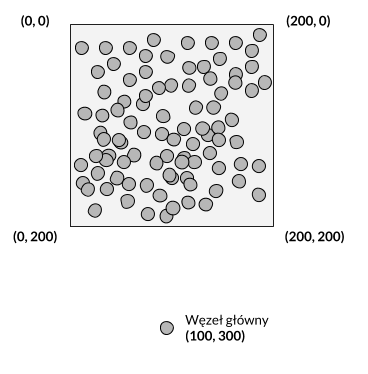
\includegraphics[width=10cm]{images/przykladowa_sieci_wygenerowana.png} 
\end{figure}

\subsection{Uruchamianie scenariuszy}

Przykład uruchamiania projektu z dwoma plikami konfiguracyjnymi:
\begin{lstlisting}
 $ /go/src/github.com/keadwen/msc_project/msc_project \
     --config_file=example1.proto,example2.proto
\end{lstlisting}

Przykład uruchamiania projektu bez pliku konfiguracyjnego:
\begin{lstlisting}
 $ /go/src/github.com/keadwen/msc_project/msc_project
\end{lstlisting}

\subsection{Generowanie wykresów}

Generowanie wykresów odbywa się przy wykorzystaniu narzędzia GNUPlot. Proces tworzenia wykresów nie jest zautomatyzowany.
Jest to dodatkowa czynność, która musi zostać wykonana manualnie po pomyślnie zakończonym procesie symulacji.
W początkowym etapie tworzenia oprogramowania, zastosowane zostało rozwiązanie przy wykorzystaniu biblioteki plotter, która
generowała dwa wykresy:

\begin{itemize}
 \item Wykres ilości aktywnych węzłów w każdej rundzie.
 \item Wykres energii całkowitej posiadanej przez wszystkie węzły w każdej rundzie.
\end{itemize}

Rozwiązanie to pomimo zalet związanych z automatycznym tworzeniem wykresów, nie pozwalało na generowanie ich w jakości spełniającej
wymagania pracy dyplomowej.

W momencie poprawnego zakończenia symulacji, folder TODO powinien posiadać zestaw plików:

% TODO: Uzupełnić w momencie tworzenia wyników do pracy.
% TODO: ls folder
\begin{lstlisting}
\end{lstlisting}

Pliki te należy następnie przekierować do GNUPlot w następujący sposób:


% TODO: Uzupełnić w momencie tworzenia wyników do pracy.
% TODO: gnuplot operations
\begin{lstlisting}
\end{lstlisting}

\subsection{Dodawanie nowych protokołów}

Architektura systemu umożliwia tworzenie nowych protokołów wymiany informacji pomiędzy węzłami.
Poprawna implementacja wymaga modifikacji oprogramowania w kilku miejscach:

\begin{enumerate}
 \item Rozszerzenie definicji enum E\_Protocol w proto/config.proto.
 \item Rozszerzenie mapProtocol w simulator/simulator.go
 \item Stworzenie nowego pliku .go w folderze core. Struktura reprezentująca nowy protokołu musi posiadać zestaw funkcji zgodny z interfejsem Protocol.
\end{enumerate}

Po wykonaniu wszystkich z powyższych kroków, protokół może zostać wykorzystany w symulacji.
Należy pamiętać, że oprogramowanie i protocol buffers będą wymagały rekompilacji. W przeciwnym wypadku zmianny nie będą widoczne.

%-----------------
% Przedstawienie i opracowanie wyników
%-----------------
\chapter{Opracowanie wyników eksperymentów}

% \section{Opis}

W tym rodziale przedstawione zostaną wyniki uzyskane w procesie symulacji przy wykorzystaniu autorskiego oprogramowania.

\section{TODO}

% TODO


\begin{thebibliography}{99}
% Bibliografia w pracy mgr jest kluczowa - powinno pojawić się kilka artykułów naukowych (IEEE, 
% ACM, Elsevier - ma Pan dostęp jako student PW)
\addcontentsline{toc}{chapter}{Bibliografia}
\bibitem{Stevens}{W. R. Stevens, G. R. Wright, ,,Biblia TCP/IP tom 1'', RM, 
1998.}
\end{thebibliography}

\zakonczenie  % wklejenie recenzji i opinii

\end{document}
%+++ END +++
